%\newcommand{\ein}[2]{(#1) (#2 Punkte)}


\begin{Large}
\textbf{Teil I: Offene Aufgaben (36 Punkte)}
\end{Large}
\\
\\
\\
\textbf{Allgemeine Anweisungen für offene Fragen:}
\\
\renewcommand{\labelenumi}{(\roman{enumi})}
\begin{enumerate}
\item
Ihre Antworten müssen alle Rechenschritte enthalten,
diese müssen klar ersichtlich sein.
Verwendung korrekter mathematischer Notation wird erwartet
und fliesst in die Bewertung ein.

\item
Ihre Antworten zu den jeweiligen Teilaufgaben müssen in den dafür vorgesehenen Platz geschrie-
ben werden. Sollte dieser Platz nicht ausreichen, setzen Sie Ihre Antwort auf der Rückseite oder
dem separat zur Verfügung gestellten Papier fort. Verweisen Sie in solchen Fällen ausdrücklich
auf Ihre Fortsetzung. Bitte schreiben Sie zudem Ihren Vor- und Nachnamen auf jeden separaten
Lösungsbogen.

\item
Es werden nur Antworten im dafür vorgesehenen Platz bewertet. Antworten auf der Rückseite
oder separatem Papier werden nur bei einem vorhandenen und klaren Verweis darauf bewertet.

\item
Die Teilaufgaben werden mit den jeweils oben auf der Seite angegebenen Punkten bewertet.

\item
Ihre endgültige Lösung jeder Teilaufgabe darf nur eine einzige Version enthalten.

\item
Zwischenrechnungen und Notizen müssen auf einem getrennten Blatt gemacht werden. Diese
Blätter müssen, deutlich als Entwurf gekennzeichnet, ebenfalls abgegeben werden.
\end{enumerate}

\newpage
\section*{\hfil Aufgaben \hfil}
\vspace{1cm}
\section*{Aufgabe 1 (35 Punkte)}
\vspace{0.4cm}
\subsection*{\aufgabe{a}{10}}
Swisslos ist in der deutschsprachigen Schweiz staatlicher Monopolist im Bereich Zahlenlottos und Sportwetten und bietet unter anderem die Produkte Swiss Lotto und Euro Millions an.
Bei einem  Verkaufspreis $ x $ pro Los der Sorte (1) Swiss Lotto und einem Verkaufspreis $ y $ pro Los der Sorte (2) Euro Millions lauten die Nachfragefunktionen:
\begin{align*}
\textrm{Nachfrage nach Swiss Lotto:} 
&\quad
q_{d_1}(x,y) = 39'500 - 1'000 x + 400y,\\
\textrm{Nachfrage nach Euro Millions:}
&\quad
q_{d_2}(x,y) = 6'500 + 300 x - 800 y.
\end{align*}
Gesucht sind die Preise $ x $ und $ y $, bei denen der Gesamtumsatz maximal ist.\\
Es wird dabei vorausgesetzt, dass die Nachfragemengen auch abgesetzt werden.\\
\\
Weisen Sie nach, dass es sich wirklich um ein Maximum handelt und berechnen Sie auch den maximalen Umsatz.
\\
\\
\subsection*{\aufgabe{b}{10}}
Gesucht ist der Punkt $ P = (x^\ast,y^\ast) $ mit $ x^\ast > 0  $ und $ y^\ast > 0 $ auf der Kurve
\begin{align*}
\varphi(x,y) = 
cx^2 +(1-c) y^2 -2 = 0, \textrm{ wobei } c \in \mathbb{R} \textrm{ mit } 0 < c < 1,
\end{align*}
sodass das Rechteck mit achsenparallelen Seiten, einer Ecke im Punkt $ (0,0) $ und der gegenüberliegenden Ecke in $ P = (x^\ast, y^\ast) $ maximale Fläche hat.\\
\\
Ermitteln Sie Kandidaten $ (x^\ast, y^\ast) $ für mögliche Maxima in Abhängigkeit des Parameters $ c $.\\
\\
\textit{Wichtige Bemerkung:}\\
Eine Abklärung, ob es sich bei den potentiellen Kandidaten um Extremstellen handelt und von welcher Art (Maxima und Minima) sie sind, wird \textbf{nicht} verlangt.
 \\
\\
\subsection*{\aufgabe{c}{5}}
Für eine Person, die am t.m.j geboren ist, sei der \glqq Geburtstagsvektor\grqq \ $ \textbf{g} = 
\begin{pmatrix}
t \\ m \\ j
\end{pmatrix}
 $.
Zum Beispiel ist der Geburtstagsvektor von Leonhard Euler, der am 15. April 1707 geboren wurde, $ \textbf{e} =
\begin{pmatrix}
15 \\ 4 \\ 1707
\end{pmatrix}
 $.
Gegeben sind die Geburtstagsvektoren von
\begin{align*}
&\textrm{Hermann Grassmann } 
\textbf{g}_1 =
\begin{pmatrix}
15 \\ 4 \\ 1809
\end{pmatrix}\\
&\textrm{William Hamilton } 
\textbf{h} =
\begin{pmatrix}
8 \\ 3 \\ 1788
\end{pmatrix}\\
&\textrm{\glqq Unbekannt\grqq } 
\textbf{u} =
\begin{pmatrix}
29 \\ m \\ 1851
\end{pmatrix}\\
&\textrm{Carl Friedrich Gauß } 
\textbf{g}_2 =
\begin{pmatrix}
30 \\ 4 \\ 1777
\end{pmatrix}
\end{align*} 
Für welche Werte von $ m \in \{1,2,3,...,12 \} $ ist es möglich, den Geburtstagsvektor von Carl Friedrich Gauß als eindeutige Linearkombination der Geburtstagsvektoren von Hermann Grassmann, William Hamilton und \glqq Unbekannt\grqq zu schreiben?
\\ \\
\subsection*{\aufgabe{d1}{6}}
Max bekommt von seinen Eltern zum 20. Geburtstag einen grosszügigen Vorschuss in Höhe von 2 Millionen Franken auf sein Erbe. Max lebt einen extravaganten Lebensstil, obwohl er bis zu seinem 20. Lebensjahr keine eigenen Ersparnisse anlegen konnte und selbst pro Jahr durch gelegentliche Arbeiten nur $ 10'000 $ Franken verdient. Er beschliesst, jedes Jahr $ 10 \% $ seines jeweiligen Vermögens auszugeben.\\
\\
Wie gross ist sein Vermögen $ V_n $ $ n $ Jahre nach seinem 20. Geburtstag, also am $ (20+ n)- $ten Geburtstag?\\
\\
Wie gross ist also sein Vermögen $ V_{10} $ am $ 30. $ Geburtstag?\\
\\
\subsection*{\aufgabe{d2}{4}}
Max bekommt von seinen Eltern zum 20. Geburtstag einen grosszügigen Vorschuss in Höhe von 2 Millionen Franken auf sein Erbe. Max lebt einen extravaganten Lebensstil, obwohl er bis zu seinem 20. Lebensjahr keine eigenen Ersparnisse anlegen konnte und selbst pro Jahr durch gelegentliche Arbeiten nur $ 10'000 $ Franken verdient. Er beschliesst, jedes Jahr $ 10 \% $ seines jeweiligen Vermögens auszugeben.\\
\\
$ V_n $ bezeichnet sein Vermögen $ n $ Jahre nach seinem 20. Geburtstag, also am $ (20+n)- $ten Geburtstag $ (n= 0,1,2,...) $.\\
\\
(\textit{Wichtige Bemerkung:} Wenn Sie Aufgabe \textbf{(d1)} nicht lösen konnten, arbeiten Sie mit $ V_n = 2 \cdot 10^6 \cdot 0.9^n+2.2 \cdot 10^5 $.)\\
\\
Welchem Wert würde sich $ V_n $ nähern, wenn Max unendlich lange leben würde?\\
\\
Wann würde sein Vermögen die Grenze von $ 500'000 $ Franken unterschreiten?
\newpage


\fancyhead[C]{\normalsize\textbf{$\qquad$ Teil II: Multiple-Choice}}
\begin{Large}
\textbf{Teil II: Multiple-Choice-Fragen (65 Punkte)}
\end{Large}
\\
\\
\\
\textbf{Allgemeine Anweisungen für Multiple-Choice-Fragen:}
\\
\renewcommand{\labelenumi}{(\roman{enumi})}
\begin{enumerate}
\item
Die Antworten auf die Multiple-Choice-Fragen müssen im dafür vorgesehenen Antwortbogen ein-
getragen werden. Es werden ausschliesslich Antworten auf diesem Antwortbogen bewertet. Der
Platz unter den Fragen ist nur für Notizen vorgesehen und wird nicht korrigiert.

\item
Jede Frage hat nur eine richtige Antwort. Es muss also auch jeweils nur eine Antwort angekreuzt
werden.

\item
Falls mehrere Antworten angekreuzt sind, wird die Antwort mit 0 Punkten bewertet, auch wenn
die korrekte Antwort unter den angekreuzten ist.

\item
Bitte lesen Sie die Fragen sorgfältig.

\end{enumerate}
\newpage
\section*{Aufgabe 2 (33 Punkte)}
\vspace{0.4cm}
\subsection*{\frage{1}{3}}
Die Funktion $ f(x,y) $ habe in $ (x_0,y_0) $ einen stationären Punkt, d.h. $ f_x(x_0,y_0)= 0 $ und $ f_y(x_0,y_0) = 0 $.\\
\\
Hinreichend dafür, dass $ f $ in $ (x_0,y_0) $ einen \textit{Sattelpunkt} hat, ist
 \renewcommand{\labelenumi}{(\alph{enumi})}
\begin{enumerate}
\item $ f_{xx}(x_0,y_0) > 0 $ und $ f_{yy}(x_0,y_0) >0 $.
\item $ f_{xx}(x_0,y_0) < 0 $ und $ f_{yy}(x_0,y_0) <0 $.
\item $ f_{xx}(x_0,y_0) > 0 $ und $ f_{yy}(x_0,y_0) <0 $.
\item Keine der vorangehenden Bedingungen ist hinreichend für einen Sattelpunkt in $ (x_0,y_0) $.
\end{enumerate}
\ \\
\subsection*{\frage{2}{3}}
Die Funktion
\begin{align*}
f(x,y) =x^2 (e^y -2) -y^2
\end{align*}
hat ein lokales Maximum in $ P = (0,0) $. Welche der folgenden Aussagen ist wahr?
\renewcommand{\labelenumi}{(\alph{enumi})}
\begin{enumerate}
\item Die Funktion $ f $ hat unter der Nebenbedingung $ \varphi(x,y)  = x^3 + 2y^4 - 4xy = 0$ ein lokales Minimum in $ P = (1,1) $.
\item Die Funktion $ f $ hat unter der Nebenbedingung $ \varphi(x,y)  = x^3 + 2y^4 - 4xy = 0$ ein lokales Maximum in $ P = (0,0) $.
\item Die Funktion $ f $ hat unter der Nebenbedingung $ \varphi(x,y)  = x^3 + 2y^4 - 4xy + 1 = 0$ ein lokales Maximum in $ P = (0,0) $.
\item Die Funktion $ f $ hat unter der Nebenbedingung $ \varphi(x,y)  = x^3 + 2y^4 - 4xy = 0$ ein lokales Minimum in $ P = (0,0) $.
\end{enumerate}
\newpage
\subsection*{\frage{3}{4}}
Die folgende Abbildung zeigt die Niveaulinien der Funktion $ f(x,y ) = 6x + 4y  $ zu verschiedenen Niveaus $ c $ und die Kurve $ \varphi(x,y) = \frac{3}{5} \ln(x) + \frac{2}{5} \ln(y) - 1 = 0 $.
\begin{center}
	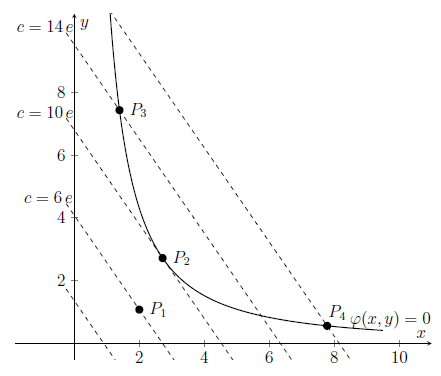
\includegraphics{pictures/frage2_3_aufgabe.png}
\end{center}
Die Funktion $ f $ hat unter der Nebenbedingung $ \varphi(x,y) = 0 $ an der Stelle
\renewcommand{\labelenumi}{(\alph{enumi})}
\begin{enumerate}
\item 
$ P_1 $ ein Minimum.
\item 
$ P_2 $ ein Minimum.
\item 
$ P_2 $ ein Maximum.
\item
$ P_4 $ ein Maximum.
\end{enumerate}
\ \\
\subsection*{\frage{4}{3}}
Die Funktion $ f $ und $ g $ schneiden sich bei $ a,\ b $ und $ c $, wobei $ a < b < c $. Zwischen $ a $ und $ b $ verläuft der Graph von $ g $ über dem Graphen von $ f $, zwischen $ b   $ und $ c $ verläuft der Graph von $ g $ unterhalb des Graphen von $ f $.\\
\\
Der Inhalt der von $ f $ und $ g $ zwischen $ a $ und $ c $ eingeschlossenen Fläche ist gleich  
\renewcommand{\labelenumi}{(\alph{enumi})}
\begin{enumerate}
	\item 
	$ \int_a^c (g(x) - f(x)) \ dx $.
	\item
	$ \int_a^b (g(x) - f(x)) \ dx - \int_b^c |g(x) - f(x)| \ dx$.
	\item
	$ \int_b^c (f(x) - g(x)) \ dx - \int_a^b (f(x) - g(x)) \ dx$.
	\item
	Keine der obigen Antworten ist korrekt.
\end{enumerate}
\ \\
\subsection*{\frage{5}{3}}
Gegeben ist die Funktion
\begin{align*}
f(x) = \int_{-1}^x \left( 2 t^2 - \frac{1}{2}t +3 \right) \ dt.
\end{align*}
Dann folgt
\renewcommand{\labelenumi}{(\alph{enumi})}
\begin{enumerate}
\item 
$ f(0) = 3 $.
\item 
$ f^\prime(0) = - \frac{1}{2} $.
\item 
$ f^{\prime \prime}(0) = - \frac{1}{2} $.
\item 
$ f^{\prime \prime \prime}(0) = 3 $.
\end{enumerate}
\ \\
\subsection*{\frage{6}{3}}
$ A $ sei eine $ (n \times m )- $Matrix, $ B $ sei eine $ (p \times q)- $Matrix.\\
Wenn die Matrix $ C = BA $ existiert, folgt:
\renewcommand{\labelenumi}{(\alph{enumi})}
\begin{enumerate}
	\item 
	$ n= q $ oder $ m = p $.
	\item 
	$ m = p $ und $ q= n $.
	\item
	$ n= p $ und $ m = q $.
	\item
	$ n = m = p = q $.
\end{enumerate}
\ \\
\subsection*{\frage{7}{4}}
Eine Matrix $ M $ heißt \textit{idempotent}, falls $ M^2 = M $ ist.\\
\\
Welche der folgenden Aussagen ist richtig?
\renewcommand{\labelenumi}{(\alph{enumi})}
\begin{enumerate}
\item 
Wenn $ M $ idempotent ist, dann folgt $ \det(M) = 1 $.
\item
$ M $ ist genau dann idempotent, wenn $ \det(M) = 0 $ oder $ \det(M) = 1 $ gilt.
\item
Wenn $ \det(M) = 0 $ ist, dann ist $ M $ idempotent.
\item
Keine der vorangehenden Aussagen ist richtig.
\end{enumerate}
\ \\
\subsection*{\frage{8}{3}}
Welche der folgenden Aussagen ist richtig für eine reellwertige Funktion $ f $?
\renewcommand{\labelenumi}{(\alph{enumi})}
\begin{enumerate}
	\item 
	Der Gradient von $ f $ in einem lokalen Extremum ist immer der Nullvektor.
	\item
	Der Gradient von $ f $ im Punkt $ (x_0,y_0) $ ist immer parallel zur Tangente an die Niveaulinie von $ f $ im Punkt $ (x_0,y_0) $.
	
	\item
	Der Vektor, der die Richtung des steilsten Abstiegs des Graphen von $ f $ im Punkt $ (x_0,y_0) $ angibt, ist parallel zur Tangenten an die Niveaulinie von $ f $ im Punkt $ (x_0,y_0) $.
	\item
	Keine der obigen Aussagen ist richtig.
\end{enumerate}
\ \\
\subsection*{\frage{9}{3}}
Welche der folgenden Behauptungen ist \textbf{nicht wahr}?
\renewcommand{\labelenumi}{(\alph{enumi})}
\begin{enumerate}
	\item 
	Das System $ \left\lbrace 
	\begin{pmatrix}
	0 \\ 1 \\ 0
	\end{pmatrix},
	\begin{pmatrix}
	2 \\ 0 \\ 2
	\end{pmatrix},
	\begin{pmatrix}
	0 \\ 0 \\ 7
	\end{pmatrix}
	\right\rbrace $
	ist linear unabhängig.
	\item
	Das System $ \left\lbrace 
	\begin{pmatrix}
	3 \\ -5 \\ 0.5
	\end{pmatrix},
	\begin{pmatrix}
	-12 \\ 20 \\ -2
	\end{pmatrix}
	\right\rbrace $
	ist linear unabhängig.
	
	\item
	Das System $ \left\lbrace 
	\begin{pmatrix}
	1 \\ 2 \\ 3
	\end{pmatrix},
	\begin{pmatrix}
	4 \\ 5 \\ 6
	\end{pmatrix},
	\begin{pmatrix}
	7 \\ 8 \\ 9
	\end{pmatrix},
	\begin{pmatrix}
	1 \\ 0 \\ 1
	\end{pmatrix}
	\right\rbrace $
	ist linear abhängig.
	\item
	Das System $ \left\lbrace 
	\begin{pmatrix}
	1 \\ 2 \\ 3
	\end{pmatrix},
	\begin{pmatrix}
	4 \\ 5 \\ 0
	\end{pmatrix},
	\begin{pmatrix}
	6 \\ 0 \\ 0
	\end{pmatrix}
	\right\rbrace $
	ist linear unabhängig.	
\end{enumerate}
\ \\
\subsection*{\frage{10}{4}}
Wir betrachten ein lineares Gleichungssystem $ A \textbf{x} = \textbf{b} $ mit $ m $ Gleichungen und $ n $ Unbekannten und $ \textbf{b} = 0 $.\\
Nachdem man den Gaußschen Algorithmus angewendet hat, bekommt man aus der erweiterten Koeffizientenmatrix $ (A | \textbf{b}) $ die neue Matrix $ (A^\ast, \textbf{b}^\ast) $, die genau $ k $ Zeilen mit lauter Nullen hat.\\
\\
Welche der folgenden Aussagen ist richtig?
\renewcommand{\labelenumi}{(\alph{enumi})}
\begin{enumerate}
	\item 
	Wenn $ k \geq 1 $ ist, dann hat das System keine Lösung.
	\item
	Wenn $ k = 1 $ ist, dann hat das System genau eine Lösung.
	
	\item
	Wenn $ k \geq 1 $ ist und $ n > m  $ ist, dann hat das System unendlich viele Lösungen, der Lösungsraum hat die Dimension $ k $.
	\item
	Wenn $ k \geq 1 $ ist und $ n > m  $ ist, dann hat das System unendlich viele Lösungen, der Lösungsraum hat die Dimension $ n+k -m$.
	
\end{enumerate}
\newpage
\section*{Aufgabe 3 (32 Punkte)}
\vspace{0.4cm}

\subsection*{\frage{1}{4}}
Gegeben ist eine Funktion $ f $ mit 
\begin{align*}
f^\prime(x) = \frac{e^x - e^{-x}}{e^x + e^{-x}} \quad \textrm{und} \quad f(0 )= 0.
\end{align*}
Dann muss gelten:
\renewcommand{\labelenumi}{(\alph{enumi})}
\begin{enumerate}
\item 
$ f(x) = \ln(e^{2x} + 1) + 2 $.
\item
$ f(x) = \ln(e^{2x} + 1) + x  - \ln(2)$.
\item
$ f(x) = \ln(e^{x} + e^{-x})  - \ln(2)$.
\item
$ f(x) = \ln(e^{x} + e^{-x})  +2$.
\end{enumerate}
\ \\
\subsection*{\frage{2}{5}}
Die stetige Zufallsvariable $ X $ hat die Dichtefunktion
\begin{align*}
f(x) =
\begin{cases}
ax + bx^2 \quad &\textrm{falls } 0 \leq x \leq 1\\
\quad  \  0 \ \ &\textrm{sonst}
\end{cases}
\end{align*}
und den Erwartungswert $ \mathbb{E}[X] = \frac{17}{24} $.\\
\\
Dann gilt:
\renewcommand{\labelenumi}{(\alph{enumi})}
\begin{enumerate}
	\item 
	$a= 6,b=-6$.
	\item
	$a= 1,b=\frac{3}{2}$.
	\item
	$a= 6,b=-5$.
	\item
	$a= \frac{3}{2},b=-\frac{1}{2}$.	
\end{enumerate}
\ \\
\subsection*{\frage{3}{4}}
Gegeben ist die Funktion
\begin{align*}
f(x,y) = 3 \ln(x^2 + y^2) - (3-a) \ln(y).
\end{align*}
Für welche $ a \in \mathbb{R} $ ist die Länge des Gradienten an der Stelle  $ (x_0,y_0) = (1,1) $ gleich $ 5 $?
\renewcommand{\labelenumi}{(\alph{enumi})}
\begin{enumerate}
\item 
$ a = \pm 4 $.
\item
$ a = \pm 2 $.
\item
$ a = \pm \sqrt{2} $.
\item
Es gibt kein solches $ a \in \mathbb{R} $.
\end{enumerate}
\ \\
\subsection*{\frage{4}{4}}
Gegeben ist die Matrix
\begin{align*}
A =
\begin{pmatrix}
2 & 4 & 6 & 8 \\
-1 & 2 & 1 & 4 \\
3 & 10 & 13 &  20 \\
4 & 0 & 4 & 0
\end{pmatrix}.
\end{align*}
$ A $ hat
\renewcommand{\labelenumi}{(\alph{enumi})}
\begin{enumerate}
\item 
den Rang $ 1 $.
\item 
den Rang $ 2 $.
\item
den Rang $ 3 $.
\item
den Rang $ 4 $.
\end{enumerate}
\ \\
\subsection*{\frage{5}{4}}
Gegeben ist die Matrix
\begin{align*}
M
=
\begin{pmatrix}
0 & 0 & -2\\
1 & 2 & 1\\
1 & 0 & 3
\end{pmatrix}.
\end{align*}
Welche der folgenden Aussagen ist richtig?
\renewcommand{\labelenumi}{(\alph{enumi})}
\begin{enumerate}
\item 
$ \textbf{x} = \begin{pmatrix}
1 \\ 0 \\ -1
\end{pmatrix} $ ist ein Eigenvektor von $ M $ zum Eigenwert $ \lambda = -2 $.
\item
$ \textbf{x} = \begin{pmatrix}
1 \\ 0 \\ 0
\end{pmatrix} $ ist ein Eigenvektor von $ M $ zum Eigenwert $ \lambda = 2 $.
\item
$ \textbf{x} = \begin{pmatrix}
-2 \\ 1 \\ 1
\end{pmatrix} $ ist ein Eigenvektor von $ M $ zum Eigenwert $ \lambda = 1 $.
\item
$ \textbf{x} = \begin{pmatrix}
1 \\ 1 \\ 1
\end{pmatrix} $ ist ein Eigenvektor von $ M $ zum Eigenwert $ \lambda = -1 $.
\end{enumerate}
\ \\
\subsection*{\frage{6}{3}}
Die Folge $ \{y_k\}_{k \in \mathbb{N}_0} $ mit $ y_k = 3 \cdot 2^k -1 $ löst die Differenzengleichung
\renewcommand{\labelenumi}{(\alph{enumi})}
\begin{enumerate}
	\item 
	$ 2 y_{k+1} - y_k = -1 $.
	\item
	$ y_{k+1} + 2 y_k  -1 = 0$.
	\item
	$ y_{k+1} + 2 y_k - 2 = 0 $.
	\item
	$ y_{k+1} - 2 y_k = 1$.
\end{enumerate}
\ \\
\subsection*{\frage{7}{3}}
Die allgemeine Lösung der Differenzengleichung
\begin{align*}
\frac{3}{4} y_k - \pi  e y_{k+1} + \frac{1}{8} y_k -3.2 = -2 y_k \quad (k=0,1,2,...)
\end{align*}
ist
\renewcommand{\labelenumi}{(\alph{enumi})}
\begin{enumerate}
\item
monoton und konvergent.
\item
monoton und divergent.	
\item 
oszillierend und konvergent.
\item
oszillierend und divergent.
\end{enumerate}
\ \\
\subsection*{\frage{8}{5}}
Die allgemeine Lösung der linearen Differenzengleichung
\begin{align*}
(a+1) y_{k+1} - (3-a) y_k + 8 = 0, \quad k = 0,1,2,...,
\end{align*}
mit $ a \in \mathbb{R} \setminus \{-1,3  \} $ ist genau dann oszillierend und konvergent, wenn
\renewcommand{\labelenumi}{(\alph{enumi})}
\begin{enumerate}
	\item 
	$ -1 < a < 1 $.
	\item
	$1 < a < 3 $.
	\item
	$ a = -1 $ oder $ a > 3 $.
	\item
	Die allgemeine Lösung ist für kein $ a \in \mathbb{R} $ oszillierend und konvergent.
\end{enumerate}